% Bolo upay — Project Report · Team WALL-E · AI Dev Fest 2026
% Build:  cd docs/report && xelatex report.tex && xelatex report.tex
\documentclass[11pt,a4paper]{article}

% ---------------------------------------------------------------- layout
\usepackage[a4paper,top=24mm,bottom=24mm,left=24mm,right=24mm,headsep=8mm,footskip=12mm]{geometry}
\usepackage{fontspec}
\setmainfont{TeX Gyre Pagella}
\setsansfont{Noto Sans}[Scale=MatchLowercase]
\setmonofont{Latin Modern Mono}[Scale=MatchLowercase]
\newfontfamily\bnfont{Noto Serif Bengali}[Script=Bengali,Scale=0.92]
\newcommand{\bn}[1]{{\bnfont #1}}

\usepackage{microtype}
\usepackage{xcolor}
\usepackage{graphicx}
\usepackage{booktabs}
\usepackage{tabularx}
\usepackage{array}
\usepackage{enumitem}
\usepackage{titlesec}
\usepackage{fancyhdr}
\usepackage{lastpage}
\usepackage{caption}
\usepackage{float}
\usepackage{needspace}
\usepackage{tikz}
\usetikzlibrary{arrows.meta,positioning,calc}
\usepackage[hidelinks]{hyperref}

\definecolor{ink}{HTML}{1B2433}
\definecolor{navy}{HTML}{0B4EA8}
\definecolor{muted}{HTML}{5F6B7A}
\definecolor{rule}{HTML}{D5DAE2}
\definecolor{panel}{HTML}{F4F6FA}
\definecolor{green}{HTML}{1E9E5A}
\definecolor{amber}{HTML}{B7791F}
\definecolor{red}{HTML}{C62828}
\color{ink}

\setlength{\parindent}{0pt}
\setlength{\parskip}{5pt}
\linespread{1.08}
\setlist{nosep,leftmargin=1.3em,topsep=3pt,itemsep=2pt}
\renewcommand{\arraystretch}{1.25}
\captionsetup{font={small,sf},labelfont={bf,color=navy},labelsep=period,justification=raggedright,singlelinecheck=false}

% headings: sans, navy, numbered, quiet
\titleformat{\section}{\sffamily\bfseries\large\color{navy}}{\thesection}{0.8em}{}
\titlespacing*{\section}{0pt}{14pt}{4pt}
\titleformat{\subsection}{\sffamily\bfseries\normalsize\color{ink}}{\thesubsection}{0.8em}{}
\titlespacing*{\subsection}{0pt}{8pt}{2pt}

% header / footer
\pagestyle{fancy}
\fancyhf{}
\renewcommand{\headrulewidth}{0.4pt}
\renewcommand{\headrule}{\hbox to\headwidth{\color{rule}\leaders\hrule height \headrulewidth\hfill}}
\fancyhead[L]{\sffamily\footnotesize\color{muted} Bolo upay \;·\; Project Report}
\fancyhead[R]{\sffamily\footnotesize\color{muted} Team WALL-E \;·\; AI Dev Fest 2026}
\fancyfoot[C]{\sffamily\footnotesize\color{muted} \thepage\ / \pageref{LastPage}}
\fancypagestyle{first}{\fancyhf{}\renewcommand{\headrulewidth}{0pt}%
  \fancyfoot[C]{\sffamily\footnotesize\color{muted} \thepage\ / \pageref{LastPage}}}

\newcommand{\metric}[2]{%
  \begin{minipage}[t]{0.235\textwidth}\centering
  {\sffamily\bfseries\fontsize{19}{22}\selectfont\color{navy}#1}\\[2pt]
  {\sffamily\scriptsize\color{muted}#2}\end{minipage}}

\begin{document}
\thispagestyle{first}

% ---------------------------------------------------------------- title block
{\sffamily\footnotesize\color{muted} AI DEV FEST 2026 \;·\; AI HACKATHON \;·\; DIU CPC $\times$ upay}\par\vspace{6pt}
{\sffamily\bfseries\fontsize{26}{30}\selectfont Bolo upay}\par\vspace{2pt}
{\sffamily\large\color{muted} A voice-first Bangla payment assistant with a scam and mistake shield}\par\vspace{10pt}

\begin{tabularx}{\textwidth}{@{}l X@{}}
\sffamily\small\color{muted} Team & \small \textbf{Team WALL-E} \,—\, Shagato Chowdhury, Umme Munia\\
\sffamily\small\color{muted} Tracks & \small 03 Customer Innovation \& Financial Independence; 01 Trust \& Risk Intelligence\\
\sffamily\small\color{muted} Repository & \small \href{https://github.com/clickTwice26/Team-WALL-E-Bolo-upay}{\texttt{github.com/clickTwice26/Team-WALL-E-Bolo-upay}}\\
\sffamily\small\color{muted} Live demo & \small \href{https://boloupay.shagato.space}{\texttt{boloupay.shagato.space}} \;(demo PIN 1234)\\
\sffamily\small\color{muted} Date & \small 4 October 2026\\
\end{tabularx}

\vspace{6pt}{\color{rule}\hrule height 0.6pt}\vspace{10pt}

% ---------------------------------------------------------------- summary
\begin{minipage}{\textwidth}
\textbf{Summary.} Stolen mobile-wallet money in Bangladesh is almost never recovered, so the only reliable moment to protect a customer is before they press send. Bolo upay lets a customer say a payment in Bangla, Banglish or English, understands it with two independent parsers that must agree, checks the transfer against the customer's own history, asks short spoken questions when something looks like a scam, and raises the authentication bar with the risk. The AI never moves money on its own.
\end{minipage}

\vspace{12pt}
\noindent\metric{91.9\%}{of scams flagged\\(rules-only baseline 53.1\%)}\hfill
\metric{1.1\%}{of honest transfers held\\(target $\le$ 2\%)}\hfill
\metric{0\%}{wrong amounts shown\\without asking}\hfill
\metric{40}{automated tests\\passing}
\par\vspace{4pt}
{\sffamily\scriptsize\color{muted} Scam-shield figures are measured on 1,200 held-out \emph{synthetic} scenarios; parser figures on 96 team-written commands. See Section~6.}

\vspace{4pt}{\color{rule}\hrule height 0.6pt}

% ---------------------------------------------------------------- 1
\section{Problem}

For upay customers who send money by phone, especially first-time and low-literate users, scams and payment mistakes cause losses that are almost never recovered. Our goal is to stop risky transfers before the money leaves, measured by scams flagged, honest transfers wrongly held, and wrong amounts shown without asking.

\begin{itemize}
  \item \textbf{Losses are not recovered.} Bangladesh Bank data reported MFS fraud of Tk 81.32 crore in 2025, of which 91.3\% was never recovered, because funds move through mule wallets within minutes. MFS fraud is more than 88\% of all unrecovered payment fraud, and officials recommended AI-driven detection~[1].
  \item \textbf{Mistakes are costly.} MFS providers handled 699,605 customer disputes worth Tk 153.98 crore in 2025~[1].
  \item \textbf{Scams work through the victim.} Most MFS fraud starts with the victim being talked into sharing a PIN or OTP, or sending money themselves~[1].
  \item \textbf{Menus exclude people.} Low-literate MFS users in Bangladesh report frequent transaction errors~[2].
  \item \textbf{Trust drives retention.} upay is a challenger with high acquisition cost (Tk 313 crore accumulated losses, 2021–2023~[3]); keeping customers active depends on trust and ease of use.
\end{itemize}

% ---------------------------------------------------------------- 2
\section{Idea}

Recovery after a scam rarely works. Bolo upay places a careful, explainable check at the moment before sending, inside a payment flow that a customer can use simply by speaking Bangla.

A mobile app cannot and should not listen to phone calls. Instead, when a transfer looks risky, the assistant \emph{asks the customer} two or three short questions aloud (``Did someone call you asking for this money?'') and checks the answers for known scam patterns. Victims usually repeat what the scammer told them, which is exactly what the check looks for.

% ---------------------------------------------------------------- 3
\section{Implemented solution}

\begin{figure}[H]
\centering
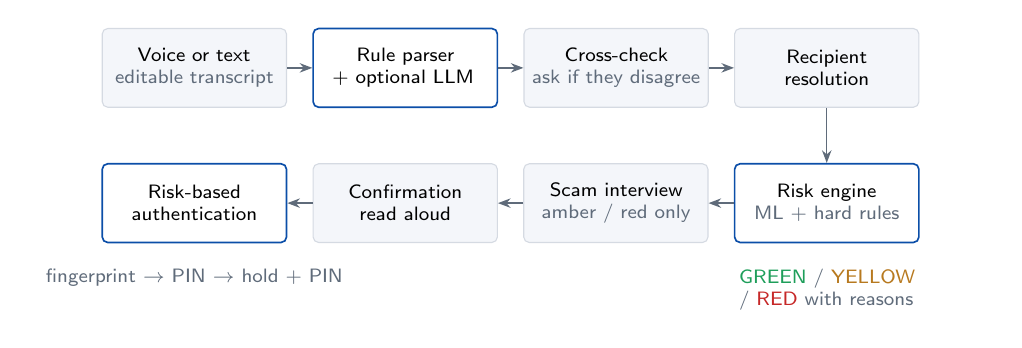
\begin{tikzpicture}[
  node distance=4mm and 3.2mm,
  box/.style={draw=rule,fill=panel,rounded corners=2pt,font=\sffamily\scriptsize,align=center,minimum height=10mm,text width=22mm,inner sep=2pt},
  key/.style={box,draw=navy,fill=white,line width=0.6pt},
  arr/.style={-{Stealth[length=1.6mm]},color=muted,line width=0.5pt}]
  \node[box] (a) {Voice or text\\ \textcolor{muted}{editable transcript}};
  \node[key,right=of a] (b) {Rule parser\\+ optional LLM};
  \node[box,right=of b] (c) {Cross-check\\ \textcolor{muted}{ask if they disagree}};
  \node[box,right=of c] (d) {Recipient\\resolution};
  \node[key,below=7mm of d] (e) {Risk engine\\ \textcolor{muted}{ML + hard rules}};
  \node[box,left=of e] (f) {Scam interview\\ \textcolor{muted}{amber / red only}};
  \node[box,left=of f] (g) {Confirmation\\read aloud};
  \node[key,left=of g] (h) {Risk-based\\authentication};
  \draw[arr] (a)--(b); \draw[arr] (b)--(c); \draw[arr] (c)--(d); \draw[arr] (d)--(e);
  \draw[arr] (e)--(f); \draw[arr] (f)--(g); \draw[arr] (g)--(h);
  \node[font=\sffamily\scriptsize,color=muted,below=2mm of h,text width=40mm,align=center] {fingerprint $\rightarrow$ PIN $\rightarrow$ hold + PIN};
  \node[font=\sffamily\scriptsize,color=muted,below=2mm of e,text width=40mm,align=center] {\textcolor{green}{GREEN} / \textcolor{amber}{YELLOW} / \textcolor{red}{RED} with reasons};
\end{tikzpicture}
\caption{Decision pipeline. Every step that can change money either asks the customer or requires their PIN or biometric.}
\end{figure}

\begin{tabularx}{\textwidth}{@{}>{\bfseries}p{30mm} X@{}}
\toprule
Flutter app & iOS, Android and Web from one codebase: PIN login, home, voice assistant, clarification, scam interview, warning and hold screens, PIN pad, Face ID / fingerprint, ops dashboard, accuracy report.\\
FastAPI backend & Parse, assess, execute, cancel, dashboard and metrics endpoints. Authentication rules are enforced on the server, not the client.\\
ML pipeline & Synthetic data generator, risk-model training with validation-tuned thresholds, parser evaluation on a labelled command set.\\
Deployment & One Docker image (API and web app on one origin) behind Caddy with automatic HTTPS.\\
\bottomrule
\end{tabularx}

% ================================================================ System design
% Included from report.tex. Notation: DeMarco/Yourdon DFD
%   external entity = rectangle, process = rounded node with number,
%   data store = open-ended box labelled D1..D5, arrows = named data flows.

\tikzset{
  ent/.style={draw=ink,line width=0.6pt,fill=white,font=\sffamily\scriptsize\bfseries,align=center,minimum width=24mm,minimum height=10mm},
  proc/.style={draw=navy,line width=0.8pt,fill=panel,rounded corners=7pt,font=\sffamily\scriptsize,align=center,minimum width=27mm,minimum height=12mm,inner sep=2pt},
  bigproc/.style={proc,minimum width=46mm,minimum height=24mm,rounded corners=14pt},
  store/.style={font=\sffamily\scriptsize,align=left,minimum width=30mm,minimum height=6mm,inner sep=2pt,
    path picture={\draw[ink,line width=0.6pt]
      (path picture bounding box.north west) -- (path picture bounding box.north east)
      (path picture bounding box.south west) -- (path picture bounding box.south east)
      ($(path picture bounding box.north west)+(6mm,0)$) -- ($(path picture bounding box.south west)+(6mm,0)$);}},
  flow/.style={-{Stealth[length=1.6mm]},color=ink!75,line width=0.5pt},
  lbl/.style={font=\sffamily\tiny,color=muted,fill=white,inner sep=1pt,align=center},
  pid/.style={font=\sffamily\tiny\bfseries,color=navy},
}
\newcommand{\pnum}[1]{{\sffamily\tiny\bfseries\color{navy}#1}\\}
\newcommand{\sid}[2]{\makebox[6mm][l]{\sffamily\bfseries #1}#2}

\section{System design}

The diagrams below describe the prototype as built. Data flow diagrams follow DeMarco notation: rectangles are external entities, rounded boxes are numbered processes, open boxes are data stores (D1–D5), and each arrow is labelled with the data it carries.

% ---------------------------------------------------------------- DFD 0
\subsection{Data flow diagram, level 0 (context)}

\begin{figure}[H]
\centering
\begin{tikzpicture}[node distance=10mm]
  \node[bigproc] (sys) {\pnum{0}\textbf{Bolo upay}\\[1pt]voice payment assistant\\with scam and mistake shield};
  \node[ent,left=34mm of sys] (cust) {Customer};
  \node[ent,right=34mm of sys] (ops) {upay operations\\team};
  \node[ent,above=14mm of sys] (llm) {LLM provider\\{\mdseries\tiny(optional)}};
  \node[ent,below=14mm of sys] (dev) {Device services\\{\mdseries\tiny speech, biometrics, call state}};

  \draw[flow] ([yshift=7mm]cust.east) -- node[lbl,above]{spoken or typed command} ([yshift=7mm]sys.west);
  \draw[flow] ([yshift=2.3mm]cust.east) -- node[lbl,above]{interview answers} ([yshift=2.3mm]sys.west);
  \draw[flow] ([yshift=-2.3mm]cust.east) -- node[lbl,below]{PIN or biometric approval} ([yshift=-2.3mm]sys.west);
  \draw[flow] ([yshift=-7mm]sys.west) -- node[lbl,below]{read-back, warnings, reasons, result} ([yshift=-7mm]cust.east);

  \draw[flow] ([yshift=4mm]sys.east) -- node[lbl,above]{decision log} ([yshift=4mm]ops.west);
  \draw[flow] ([yshift=-4mm]sys.east) -- node[lbl,below]{dashboard and accuracy metrics} ([yshift=-4mm]ops.west);

  \draw[flow] ([xshift=-6mm]sys.north) -- node[lbl,left]{command text} ([xshift=-6mm]llm.south);
  \draw[flow] ([xshift=6mm]llm.south) -- node[lbl,right]{structured intent} ([xshift=6mm]sys.north);

  \draw[flow] ([xshift=-6mm]dev.north) -- node[lbl,left]{transcript, call state} ([xshift=-6mm]sys.south);
  \draw[flow] ([xshift=6mm]sys.south) -- node[lbl,right]{speech prompts} ([xshift=6mm]dev.north);
\end{tikzpicture}
\caption{Context diagram. Raw audio stays on the device: only the transcript reaches the system. Phone calls are never recorded; at most the native app learns that a call is active.}
\end{figure}

% ---------------------------------------------------------------- DFD 1
\clearpage
\subsection{Data flow diagram, level 1}

\begin{figure}[H]
\centering
\begin{tikzpicture}[scale=0.94,transform shape]
  % processes
  \node[proc] (p1) at (0,0)      {\pnum{1.0}Understand\\command};
  \node[proc] (p2) at (4.6,0)    {\pnum{2.0}Resolve\\recipient};
  \node[proc] (p3) at (9.2,0)    {\pnum{3.0}Assess\\risk};
  \node[proc] (p4) at (9.2,-4.5) {\pnum{4.0}Scam\\interview};
  \node[proc] (p5) at (4.6,-4.5) {\pnum{5.0}Authenticate\\and execute};
  \node[proc] (p6) at (0,-4.5)   {\pnum{6.0}Report and\\monitor};
  % external entities
  \node[ent] (cust) at (0,3) {Customer};
  \node[ent] (llm)  at (4.6,3) {LLM provider};
  \node[ent] (ops)  at (0,-8.2) {upay operations\\team};
  % data stores
  \node[store] (d1) at (4.6,-2.25)  {\sid{D1}Users and contacts};
  \node[store] (d5) at (12.9,0.3)   {\sid{D5}Lexicon, model};
  \node[store] (d2) at (12.9,-2.25) {\sid{D2}Transactions};
  \node[store] (d3) at (12.9,-4.5)  {\sid{D3}Assessments};
  \node[store] (d4) at (4.6,-6.8)   {\sid{D4}Decision log};

  % customer and LLM
  \draw[flow] ([xshift=-4mm]cust.south) -- node[lbl,left]{command text} ([xshift=-4mm]p1.north);
  \draw[flow] ([xshift=4mm]p1.north) -- node[lbl,right]{question} ([xshift=4mm]cust.south);
  \draw[flow] ([yshift=4.5mm]p1.east) -- node[lbl,above,sloped]{text} ([yshift=-1mm]llm.west);
  \draw[flow] ([yshift=-4mm]llm.west) -- node[lbl,below,sloped]{intent JSON} ([yshift=1.5mm]p1.east);
  % main path
  \draw[flow] ([yshift=-2mm]p1.east) -- node[lbl,below]{intent, amount} ([yshift=-2mm]p2.west);
  \draw[flow] (p2.east) -- node[lbl,above]{draft transfer} (p3.west);
  \draw[flow] (d1.north) -- node[lbl,right]{contacts} (p2.south);
  \draw[flow] (d1.south) -- node[lbl,right]{balance} (p5.north);
  \draw[flow] (d5.west) -- node[lbl,above]{weights} ([yshift=3mm]p3.east);
  \draw[flow] (d2.north) |- node[lbl,pos=0.75,below]{history} ([yshift=-3mm]p3.east);
  \draw[flow] ([xshift=-4mm]p3.south) -- node[lbl,left]{amber/red: questions} ([xshift=-4mm]p4.north);
  \draw[flow] ([xshift=4mm]p4.north) -- node[lbl,right]{answers} ([xshift=4mm]p3.south);
  \draw[flow] (p3.south west) -- node[lbl,above,sloped]{green: level, auth} (p5.north east);
  \draw[flow] (p4.west) -- node[lbl,above]{level, reasons} (p5.east);
  \draw[flow] (p4.east) -- node[lbl,above]{assessment} (d3.west);
  \draw[flow] (cust.west) -- ++(-0.6,0) |- node[lbl,pos=0.75,above]{PIN / biometric} (p5.north west |- 0,-3.1) -- ([xshift=-6mm]p5.north);
  \draw[flow] ([xshift=8mm]p5.south) |- (14.7,-5.7) |- node[lbl,pos=0.25,right]{new transaction} (d2.east);
  \draw[flow] (p5.south) -- node[lbl,right]{decision} (d4.north);
  \draw[flow] (d4.west) -| node[lbl,pos=0.25,above]{log} ([xshift=6mm]p6.south);
  \draw[flow] ([xshift=-6mm]p6.south) -- node[lbl,left]{dashboard, metrics} ([xshift=-6mm]ops.north);
\end{tikzpicture}
\caption{Level 1. Process 3.0 never moves money; only 5.0 does, and only after the customer's PIN or biometric. Process 4.0 runs only when 3.0 rates a transfer amber or red.}
\end{figure}

\begin{tabularx}{\textwidth}{@{}>{\sffamily\bfseries\small}p{10mm} >{\raggedright\arraybackslash}p{36mm} X@{}}
\toprule
\textnormal{\sffamily\small No.} & \sffamily\small Process & \sffamily\small What it does\\
\midrule
1.0 & Understand command & Normalises Bangla digits and number words, extracts intent, amount and phone number; compares with the optional LLM and asks if they disagree.\\
2.0 & Resolve recipient & Matches names and nicknames against D1 with Bangla case suffixes; ambiguous or fuzzy matches go back to the customer.\\
3.0 & Assess risk & Computes features from D2, matches scam phrases, scores with the model in D5, applies hard rules and the mistake guard (see level 2).\\
4.0 & Scam interview & Asks up to three spoken questions and sends the answers back to 3.0 for a second assessment, stored in D3.\\
5.0 & Authenticate and execute & Enforces biometric, PIN or hold-then-PIN by level; writes the transfer to D2 and the outcome to D4.\\
6.0 & Report and monitor & Aggregates D4 into the ops dashboard and serves the measured accuracy figures.\\
\bottomrule
\end{tabularx}

% ---------------------------------------------------------------- DFD 2
\clearpage
\subsection{Data flow diagram, level 2: process 3.0 Assess risk}

\begin{figure}[H]
\centering
\begin{tikzpicture}[scale=0.94,transform shape]
  \node[ent,dashed] (in)  at (0,0)     {from 2.0\\{\mdseries\tiny draft transfer}};
  \node[ent,dashed] (ans) at (0,-3.6)  {from 4.0\\{\mdseries\tiny interview answers}};
  \node[proc] (q1) at (4.6,0)    {\pnum{3.1}Compute\\features};
  \node[proc] (q2) at (4.6,-3.6) {\pnum{3.2}Match scam\\phrases};
  \node[proc] (q3) at (9.4,-1.8) {\pnum{3.3}Score with\\model};
  \node[proc] (q4) at (9.4,-5.4) {\pnum{3.4}Hard rules and\\mistake guard};
  \node[proc] (q5) at (13.8,-3.6){\pnum{3.5}Decide level\\and reasons};
  \node[store] (d1) at (2.9,2.3)   {\sid{D1}Users, contacts};
  \node[store] (d2) at (6.6,2.3)   {\sid{D2}Transactions};
  \node[store] (d5m) at (9.4,0.6)  {\sid{D5}Risk model};
  \node[store] (d5) at (4.6,-6.2)  {\sid{D5}Scam lexicon};
  \node[store] (d3) at (13.8,-7.0) {\sid{D3}Assessments};
  \node[ent,dashed] (out) at (13.8,0.2) {to 4.0 or 5.0\\{\mdseries\tiny level, reasons, auth}};

  \draw[flow] (in) -- node[lbl,above]{amount, recipient} (q1);
  \draw[flow] (d1.south) -- node[lbl,left]{contacts, balance} (q1.north west);
  \draw[flow] (d2.south) -- node[lbl,right]{history} (q1.north east);
  \draw[flow] (in.south east) -- node[lbl,above,sloped]{command text} (q2.north west);
  \draw[flow] (ans) -- node[lbl,above]{answers} (q2);
  \draw[flow] (d5.north) -- node[lbl,right]{lexicon} (q2.south);
  \draw[flow] (d5m.south) -- node[lbl,right]{weights, thresholds} (q3.north);
  \draw[flow] (q1.east) -- node[lbl,above,sloped]{9 features} (q3.north west);
  \draw[flow] (q2.north east) -- node[lbl,below,sloped]{scam score} (q3.south west);
  \draw[flow] (q2.south east) -- node[lbl,below,sloped]{categories} (q4.west);
  \draw[flow] (q1.south east) -- node[lbl,pos=0.78,above,sloped]{inflow, usual amount} (q4.north west);
  \draw[flow] (q3.east) -- node[lbl,above,sloped]{probability} (q5.north west);
  \draw[flow] (q4.east) -- node[lbl,below,sloped]{overrides, suggestion} (q5.south west);
  \draw[flow] (q5.north) -- (out.south);
  \draw[flow] (q5.south) -- node[lbl,right]{stored assessment} (d3.north);
\end{tikzpicture}
\caption{Level 2 of process 3.0. Hard rules (3.4) override the model: a PIN or OTP request, a ``send it back'' claim with no incoming money, or a ``relative in trouble'' story from a new number always yields red.}
\end{figure}

\begin{tabularx}{\textwidth}{@{}>{\sffamily\bfseries\small}p{10mm} X@{}}
\toprule
3.1 & New recipient, amount relative to what this person usually receives, share of balance, sends in the last 30 minutes, night time, active call, refund claim without incoming money.\\
3.2 & Each utterance is matched separately against eight scam categories in Bangla, Banglish and English; a following negation (\bn{না}, \bn{চায়নি}, ``nai'') cancels a match.\\
3.3 & Logistic regression; probability compared with thresholds tuned on validation data (amber $\ge$ 0.08, red $\ge$ 0.90).\\
3.4 & Unambiguous evidence forces red; a known recipient receiving about ten times the usual amount triggers ``Did you mean \dots?''\\
3.5 & Combines the above into green, amber or red, the reasons shown to the customer, the required authentication, and whether to run the interview.\\
\bottomrule
\end{tabularx}

% ---------------------------------------------------------------- sequence
\clearpage
\subsection{Sequence diagram: a scam attempt that is stopped}

\begin{figure}[H]
\centering
\begin{tikzpicture}[
  msg/.style={-{Stealth[length=1.5mm]},line width=0.5pt,color=ink},
  ret/.style={-{Stealth[length=1.5mm]},line width=0.5pt,color=muted,dashed},
  mt/.style={font=\sffamily\tiny,above,inner sep=1pt,fill=white},
  head/.style={draw=ink,line width=0.6pt,fill=panel,font=\sffamily\scriptsize\bfseries,minimum width=21mm,minimum height=8mm,align=center},
  act/.style={draw=navy,fill=navy!12,minimum width=2mm,inner sep=0}]
  % lifelines
  \foreach \x/\n/\t in {0/C/Customer,2.75/A/Flutter app,5.5/P/API,8.25/R/Parser\\{\mdseries\tiny + optional LLM},11/K/Risk engine,13.75/S/Store\\{\mdseries\tiny D1--D4}} {
    \node[head] (\n) at (\x,0) {\t};
    \draw[color=rule,line width=0.6pt,dashed] (\x,-0.5) -- (\x,-19.4);
  }
  \newcommand{\sqm}[4]{\draw[msg] (#1,#3) -- node[mt]{#4} (#2,#3);}
  \newcommand{\sqr}[4]{\draw[ret] (#1,#3) -- node[mt]{#4} (#2,#3);}
  \newcommand{\sqnote}[2]{\node[font=\sffamily\tiny\bfseries,color=navy,anchor=west] at (-0.6,#1) {#2};}

  \sqnote{-0.95}{1\; Command}
  \sqm{0}{2.75}{-1.4}{``01799998888 e 5000 taka pathao''}
  \sqm{2.75}{5.5}{-2.0}{POST /api/parse}
  \sqm{5.5}{8.25}{-2.6}{parse(text)}
  \sqr{8.25}{5.5}{-3.2}{send\_money, 5000, new number}
  \sqr{5.5}{2.75}{-3.8}{status ok}

  \sqnote{-4.35}{2\; First risk check}
  \sqm{2.75}{5.5}{-4.8}{POST /api/assess (on call)}
  \sqm{5.5}{13.75}{-5.4}{load history, contacts, balance}
  \sqr{13.75}{5.5}{-6.0}{}
  \sqm{5.5}{11}{-6.6}{features, score}
  \sqr{11}{5.5}{-7.2}{AMBER, interview needed}
  \sqr{5.5}{2.75}{-7.8}{3 questions}

  \sqnote{-8.35}{3\; Scam interview}
  \sqr{2.75}{0}{-8.8}{``Did someone call you asking for this money?''}
  \sqm{0}{2.75}{-9.4}{``\bn{উপায় অফিস থেকে ফোন দিয়েছে}''}
  \sqm{2.75}{5.5}{-10.0}{POST /api/assess + answers}
  \sqm{5.5}{11}{-10.6}{match phrases, rules}
  \sqr{11}{5.5}{-11.2}{RED: fake upay staff}
  \sqm{5.5}{13.75}{-11.8}{save assessment (D3)}
  \sqr{5.5}{2.75}{-12.4}{RED, reasons, hold 30 s}

  \sqnote{-12.95}{4\; Warning and decision}
  \sqr{2.75}{0}{-13.4}{warning read aloud, helpline 16268}
  \sqm{0}{2.75}{-14.0}{Cancel}
  \sqm{2.75}{5.5}{-14.6}{POST /api/cancel}
  \sqm{5.5}{13.75}{-15.2}{log ``cancelled after warning'' (D4)}
  \sqr{5.5}{2.75}{-15.8}{ok}
  \sqr{2.75}{0}{-16.4}{``Cancelled. Your money is safe.''}

  \node[draw=rule,fill=panel,font=\sffamily\tiny,align=left,text width=60mm,anchor=north west] at (0.6,-17.0)
    {\textbf{If the customer continues instead:} the app waits for the hold to end, requires the warning to be acknowledged and the PIN to be entered; the server re-checks all three before \texttt{/api/execute} writes the transfer. Biometrics are refused for amber and red.};
  % activations
  \node[act,minimum height=33mm,anchor=north] at (5.5,-1.9) {};
  \node[act,minimum height=26mm,anchor=north] at (5.5,-9.9) {};
\end{tikzpicture}
\caption{Sequence of a fake-upay-staff scam: the first check finds a new number, a large share of the balance and an active call; the customer's own answer confirms the pattern; the transfer is held and cancelled before any money moves.}
\end{figure}


% ---------------------------------------------------------------- 4
\clearpage
\section{Key features}

\begin{enumerate}
  \item \textbf{Natural commands.} Bangla, Banglish and English, including Bangla number words (\bn{দেড় হাজার} = 1,500, \bn{আড়াইশো} = 250, \bn{সাড়ে তিন হাজার} = 3,500, \bn{পৌনে দুই হাজার} = 1,750), Bangla digits, ``5k'' and spoken phone numbers.
  \item \textbf{Never guesses money or people.} Two possible amounts, two contacts named Rahim, or a misheard name all lead to a question, not a guess.
  \item \textbf{Scam shield.} Three levels with plain-Bangla reasons for every warning.
  \item \textbf{Spoken scam interview} with negation handling (``nobody asked for my OTP'' is not a scam signal).
  \item \textbf{Hard rules for clear evidence}, e.g.\ a request to ``send it back'' when no money ever arrived from that number.
  \item \textbf{Mistake guard.} ``You usually send this person about Tk 360. Did you mean Tk 350?''
  \item \textbf{Risk-based authentication.} Biometric only for low risk; PIN for medium; a 30-second hold, warning acknowledgement and PIN for high risk.
  \item \textbf{Ops dashboard and in-app accuracy report} showing transfers cancelled after a warning and money protected.
\end{enumerate}

% ---------------------------------------------------------------- 5
\section{AI approach}

\begin{tabularx}{\textwidth}{@{}>{\raggedright\arraybackslash\bfseries}p{24mm} >{\raggedright\arraybackslash}X >{\raggedright\arraybackslash}p{50mm}@{}}
\toprule
\textnormal{\sffamily\small Part} & \sffamily\small Method & \sffamily\small Reason\\
\midrule
Speech & On-device speech-to-text; transcript always editable & Recognition makes mistakes; the user can fix the text\\
Parsing & Deterministic Bangla/Banglish/English parser plus optional LLM (Gemini, OpenAI or Claude) with structured output; disagreement leads to a question & Money needs a second opinion; rules are predictable, the LLM covers unusual phrasing\\
Recipient & Alias matching with Bangla case suffixes; longest alias wins; fuzzy matches need confirmation & Real contact lists have duplicates and nicknames\\
Risk score & Logistic regression on nine history features & AUC close to gradient boosting (0.986 vs 0.992) and fully explainable\\
Thresholds & Tuned on a validation split: honest transfers held $\le$ 2\%, then maximise scams flagged & Limits friction for honest customers explicitly\\
Scam phrases & Lexicon of 8 scam types in three languages; exact and fuzzy matching; negation-aware & Victims repeat what the scammer said\\
Evaluation & Two-stage (command only, then with interview answers); 70/15/15 split; rules-only baseline & Mirrors how the app actually decides\\
\bottomrule
\end{tabularx}

\subsection{Model features and learned weights}
\begin{tabularx}{\textwidth}{@{}>{\ttfamily\small}p{46mm} X r@{}}
\toprule
\textnormal{\sffamily\small Feature} & \sffamily\small Meaning & \sffamily\small Weight\\
\midrule
scam\_score & Scam phrases in the command or interview answers & 1.90\\
balance\_fraction & Share of the balance being sent & 1.69\\
is\_new\_recipient & Never sent to before and not in contacts & 1.50\\
on\_active\_call & A phone call is active (native signal; simulated in the prototype) & 0.80\\
recent\_sends\_30m & Number of sends in the last 30 minutes & 0.72\\
return\_claim\_no\_inflow & ``Send it back'' but nothing arrived from that number (also a hard rule) & 0.49\\
is\_night & Between 00:00 and 05:00, Dhaka time & 0.18\\
log\_recipient\_ratio & Amount relative to what this person usually receives & 0.04\\
is\_recharge & Mobile recharge rather than send money & $-$0.33\\
\bottomrule
\end{tabularx}

% ---------------------------------------------------------------- 6
\Needspace{12\baselineskip}
\section{Results}

\subsection{Command understanding}
96 labelled commands written by the team (Bangla, Banglish, English, Bangla digits, number words, phone numbers, ambiguous names and amounts), rule parser only.

\begin{tabularx}{\textwidth}{@{}X r X r@{}}
\toprule
Intent accuracy & 100\% & Recipient accuracy & 100\%\\
Amount accuracy & 100\% & Wrong amount shown without asking & \textbf{0\%}\\
\bottomrule
\end{tabularx}

\subsection{Scam shield}
1,200 held-out synthetic scenarios (309 scams, 891 honest transfers); thresholds chosen on a separate validation split.

\begin{tabularx}{\textwidth}{@{}X r r@{}}
\toprule
\sffamily\small Measure & \sffamily\small Bolo upay & \sffamily\small Rules only\\
\midrule
Scams flagged (yellow or red) & \textbf{91.9\%} & 53.1\%\\
Scams held at red & \textbf{73.8\%} & 16.2\%\\
Honest transfers held at red & 1.1\% & 0.9\%\\
Honest transfers asked for PIN with a warning & 13.4\% & 6.1\%\\
\bottomrule
\end{tabularx}

\vspace{2pt}
{\small\color{muted} The scenarios are simulated because no real fraud data is available to the team; they show that the pipeline behaves as designed, not real-world fraud performance. The parser test set was written alongside the parser, so real speech will be harder.}

% ---------------------------------------------------------------- 7
\Needspace{8\baselineskip}
\section{Real-life impact}

\begin{itemize}
  \item \textbf{Customers.} A ten-second pause with the right question at the right moment, in their own language. Scam victims are stopped before the money leaves.
  \item \textbf{upay.} Fewer disputes from wrong-number and wrong-amount transfers; lower fraud loss and reputational damage; a clear difference from competitors; voice access for customers who avoid the app today.
  \item \textbf{Pilot metrics.} Scams cancelled after a warning, money protected, disputes per 10,000 transfers, false-alarm rate, and voice-command completion rate.
\end{itemize}

% ---------------------------------------------------------------- 8
\section{Responsible AI and security}

Synthetic data only, with no personal information. No call recording and no voice biometrics, since voices can be cloned. The AI never moves money: every transfer needs the customer's PIN or biometric, and the server decides which is required. PINs are hashed; three wrong attempts lock the transaction. Every warning is explained, and false alarms are measured and reported so thresholds can be chosen to limit them.

% ---------------------------------------------------------------- 9
\section{Limitations and next steps}

\begin{tabularx}{\textwidth}{@{}>{\raggedright\arraybackslash}X >{\raggedright\arraybackslash}X@{}}
\toprule
\sffamily\small Limitation & \sffamily\small Next step\\
\midrule
Model trained on synthetic data & Validate on governed, anonymised upay data\\
Test commands written by the team & Collect real Bangla voice commands from consenting pilot users\\
Bangla speech recognition varies by device & Compare on-device and server speech recognition\\
A pressured victim can ignore a warning & Delayed release or call-back for very risky transfers\\
Account takeover and USSD users not covered & SMS confirmation path for USSD; device and login security\\
Call-state signal is simulated & Implement in the native app with the customer's permission\\
\bottomrule
\end{tabularx}

\subsection{Path to production}
Competition review $\rightarrow$ technical and business review $\rightarrow$ controlled validation on governed data $\rightarrow$ proof of concept inside the upay app (send money only) $\rightarrow$ pilot with first-time users $\rightarrow$ measure scams stopped, disputes, false alarms and completion rate $\rightarrow$ integrate.

% ---------------------------------------------------------------- screens
\clearpage
\section{Prototype screens}

\begin{figure}[H]
\centering
\newcommand{\shot}[2]{\begin{minipage}[t]{0.185\textwidth}\centering
  \includegraphics[width=\linewidth]{../screenshots/#1}\\[2pt]{\sffamily\scriptsize\color{muted}#2}\end{minipage}}
\shot{00_login.png}{PIN login}\hfill
\shot{01_home.png}{Home}\hfill
\shot{03_green.png}{Normal send}\hfill
\shot{09_pin.png}{PIN}\hfill
\shot{10_done.png}{Done}\\[10pt]
\shot{04_which_rahim.png}{Which Rahim?}\hfill
\shot{05_extra_zero.png}{Extra zero}\hfill
\shot{06_interview.png}{Scam interview}\hfill
\shot{07_red.png}{Fake upay call}\hfill
\shot{08_hold.png}{Hold before PIN}
\caption{Screens from the running prototype (web build). A ribbon on every screen marks it as a prototype, not the official upay app.}
\end{figure}

% ---------------------------------------------------------------- refs
\section*{References}
\small
\begin{enumerate}[label={[\arabic*]},leftmargin=2em]
  \item New Age, ``Over 90pc stolen funds from MFS remain unrecovered,'' 3 July 2026 (Bangladesh Bank data).
  \item ``Smartphone based Inclusive MFS Design for Low-Literate Population,'' ACM Digital Library.
  \item The Business Standard, ``upay's accumulated losses cross Tk300cr in 2023,'' 15 June 2024.
\end{enumerate}

\vspace{4pt}
{\footnotesize\color{muted} Disclosure: AI coding assistants were used during development, as permitted by the competition rules. All users, phone numbers and transactions in the prototype are synthetic.}

\end{document}
